{\bfseries 根据上述三个纠正后的模型得到如下模型结果:}
\begin{figure}[h!]
	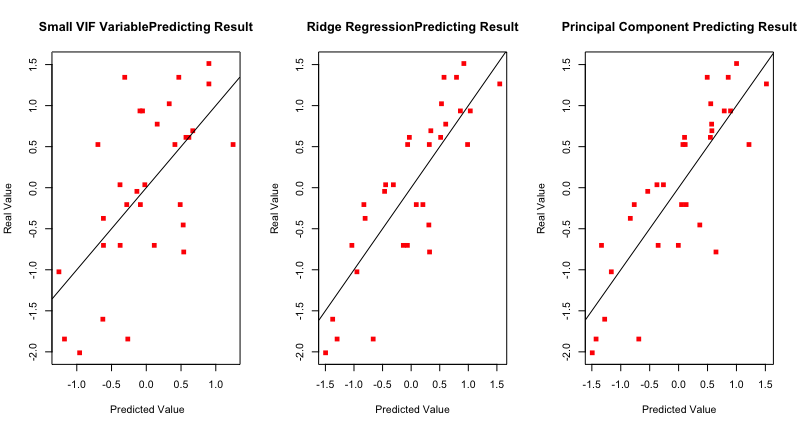
\includegraphics[width=10cm]{Conclusion.png}
	\centering
	\caption{预测结果}
	\label{fig:18}
\end{figure}
看出通过第一种纠正方式,即简单除去膨胀因子过大的变量,导致预测值和真实值在$y=x$两侧的离散程度较大,三个图中,岭回归模型预测的结果是最优的。
比较三组纠正模型的MSE值可得到:
\begin{table}[h]
	\begin{tabular}{|c|c|c|}
		\hline
		Small VIF Variable& Ridge Regression &Principal Component Regression\\
		0.738011&0.5321579&0.5543356\\
		\hline
	\end{tabular}
\centering
\end{table}
由上表结论可知,岭回归模型在这里的表现最好,本文采用岭回归模型进行预测NBA球员数据和球队胜率的关系会得到更好的结果。\\



{\bfseries 模型评价:}由于本文试图通过公开的数据和建模寻找球员表现和球队胜负的关系,其中一些不可控因素会导致模型出现一定的问题,例如,一些球员在赛季中受伤退赛或者没有退赛但是伤势会对其表现有很大的影响;或者某些球员在某一赛季中因选秀被交易到其他球队效力;或者某队在赛季中因更换教练导致球队风格有了很大的改变;或者某些球队的数据过于相似而导致其特征不够显著而无法得到更精准的预测。\cite{yang2015predicting}
\\
此外我们得到我们的变量对因变量具有一定的解释作用,其中球员实际命中率每增加1\%,球队的胜率会降低0.42\%,
球员有效得分率每提高1\%,球队获胜的概率会上升0.71\%,球员使用率每上升1\%,就会对球队造成胜率下降0.63\%的影响,而球员效率每提高1\%就会对球队获胜的概率提升0.48\%,球队控球时间越长就会对球队的胜率影响不利;该模型说明,当球队在制定训练方案时应着重注意的是提升球员的个人效率,降低球队对每位球员的使用效率,不仅要提高球员的投篮命中率,还有增强球员之间的团结合作,提升有效得分率。最终要严格控制每场比赛球队在场上的控球时间,这样可以节省运动员体能,获得更精彩的发挥。